\section{Research Papers}
\label{sec:research-papers}

\subsection{Debugging of RxJS-Based Applications}
\label{sec:paper-1}

This paper was published with the proceedings of the 7th ACM SIGPLAN International Workshop
on Reactive and Event-Based Languages and Systems (REBLS '20), 16th November 2020.

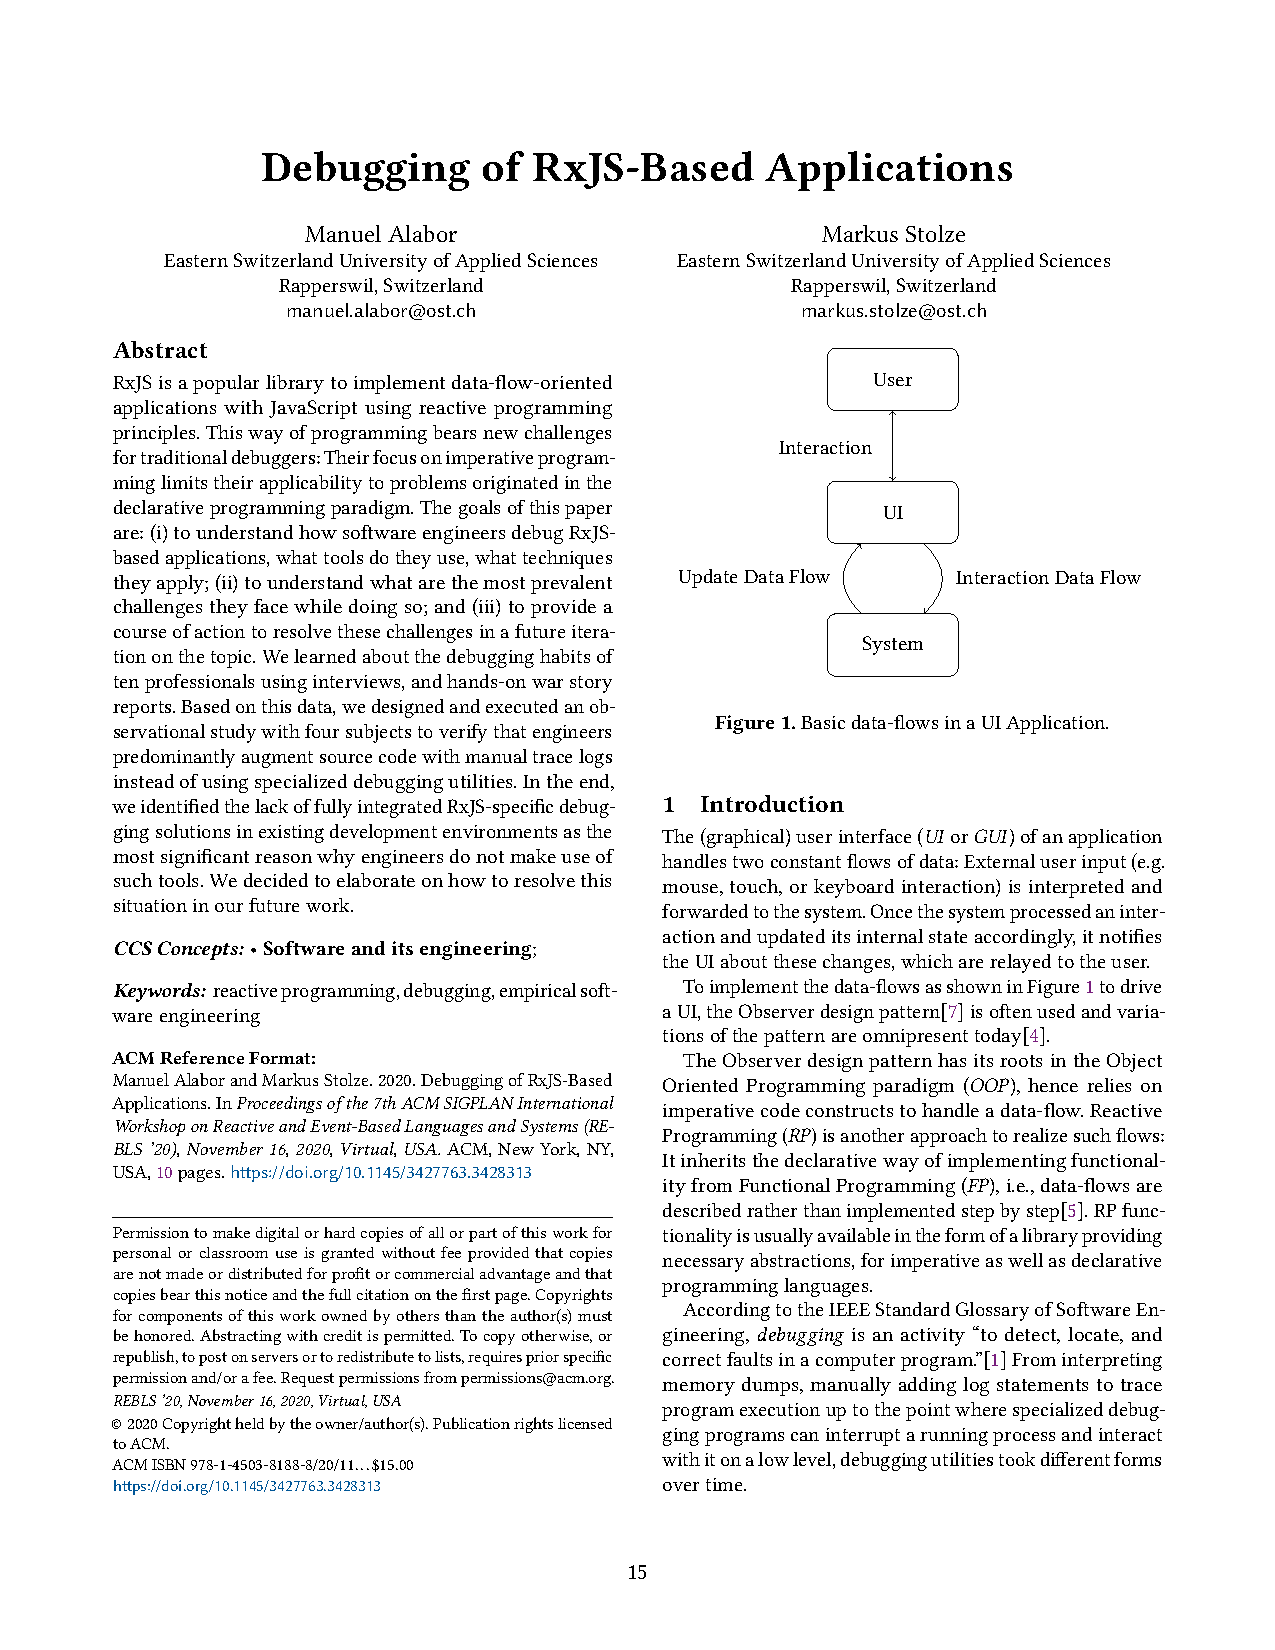
\includepdf[pages=-]{content/pdfs/3427763.3428313.pdf}



\subsection{Debugging Support for Reactive Programming}
\label{sec:paper-2}

The review version of this paper (Appendix \ref{sec:paper-2-paper}) and its supplementary material
(Appendix \ref{sec:paper-2-supplementary}) were submitted to the Technical Papers track at the 31st ACM SIGSOFT
International Symposium on Software Testing and Analysis 2022 (ISSTA '22).

\subsubsection{Paper}
\label{sec:paper-2-paper}
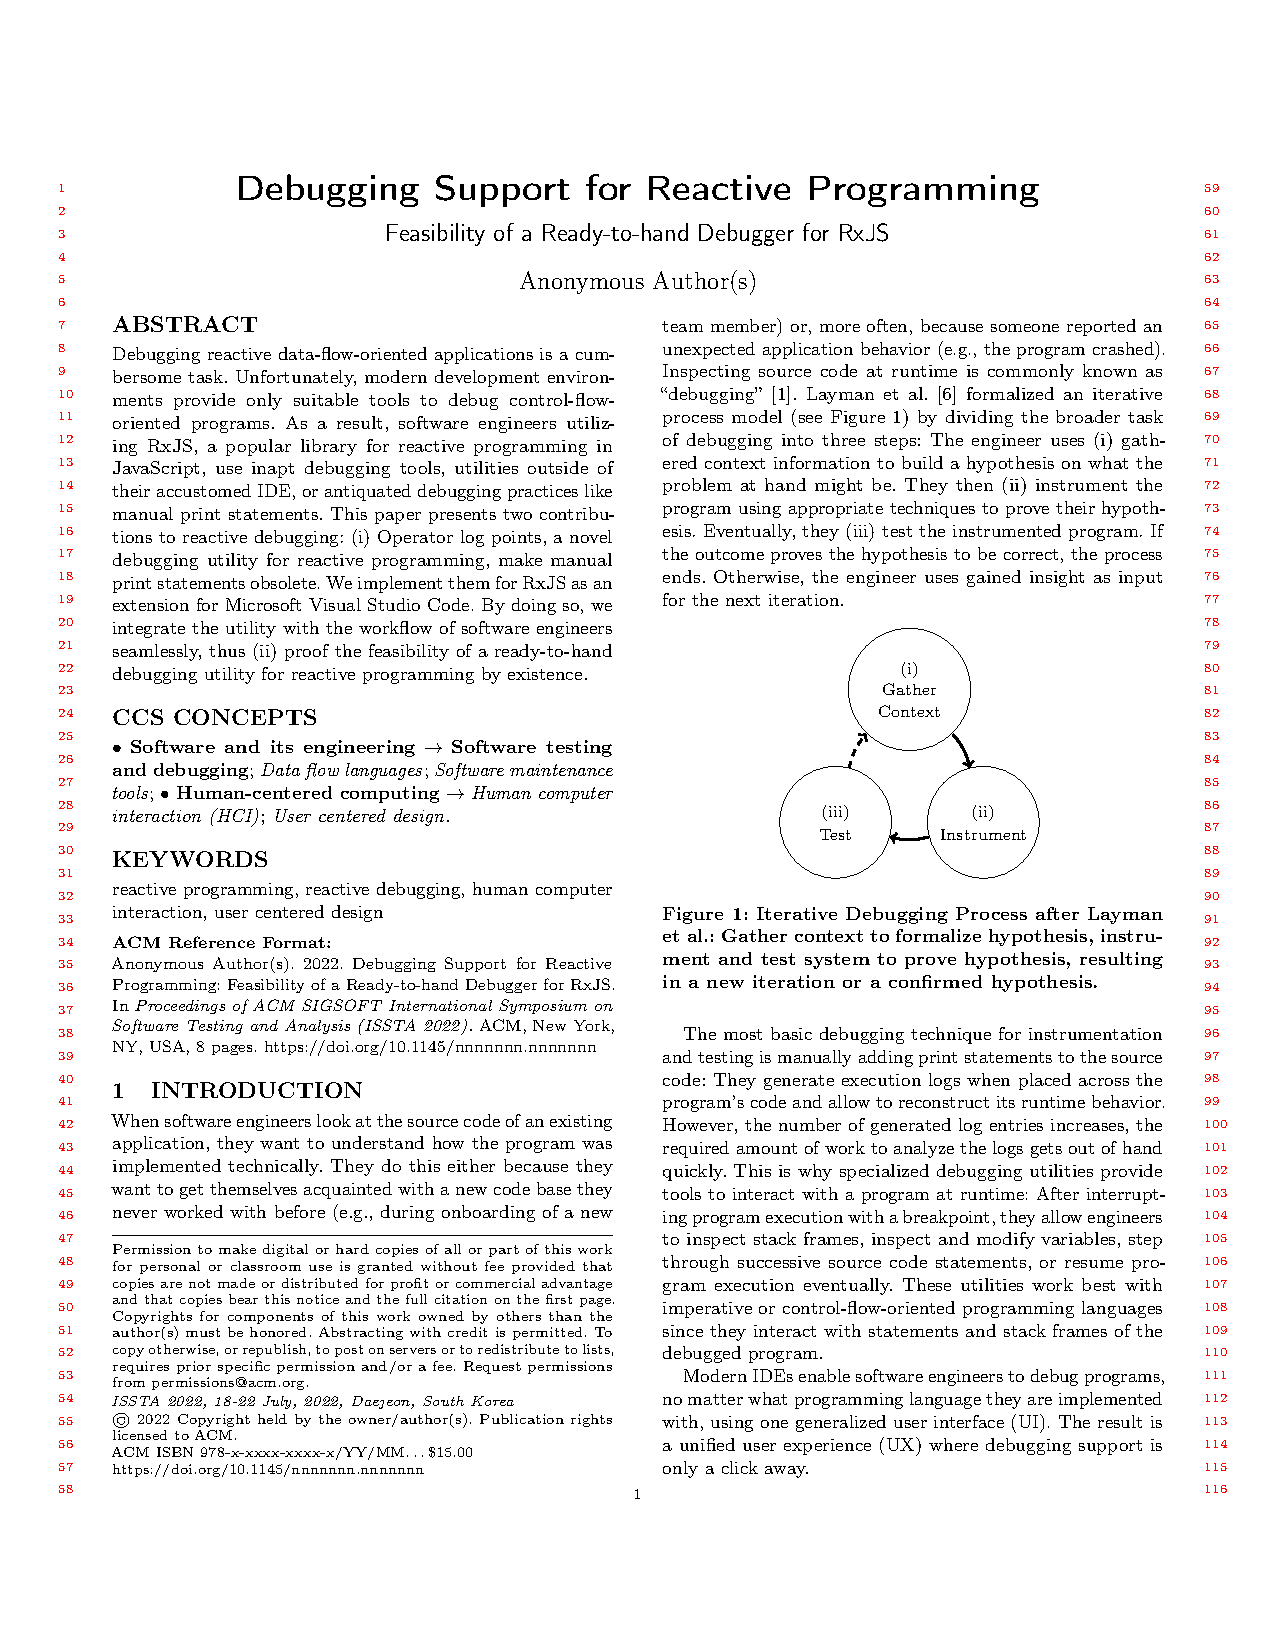
\includepdf[pages=-]{content/pdfs/issta/paper.pdf}

\subsubsection{Supplementary Material}
\label{sec:paper-2-supplementary}
\includepdf[pages=1-12]{content/pdfs/issta/supplementary-material.pdf}
\includepdf[pages=13-14,landscape=true]{content/pdfs/issta/supplementary-material.pdf}
\includepdf[pages=15-]{content/pdfs/issta/supplementary-material.pdf}


\section{Comparative User Journey}
\label{sec:user-journey}

The Comparative User Journey is publicly accessible on alabor.me and GitHub as well:

\begin{itemize}
  \item \url{https://alabor.me/research/user-journey-debugging-of-rxjs-based-applications/}
  \item \url{https://github.com/swissmanu/alabor.me/tree/master/research/user-journey-debugging-of-rxjs-based-applications}
\end{itemize}


\includepdf[pages=-]{content/pdfs/user-journey.pdf}



\section{RxJS Debugging for vscode}


\subsection{Major Release Milestone Plan}
\label{sec:major-milestone}
The following document was created at the 31th of December, 10:00 CET and is publicly accesible:

\begin{itemize}
  \item \url{https://github.com/swissmanu/rxjs-debugging-for-vscode/milestone/2?closed=1}
\end{itemize}

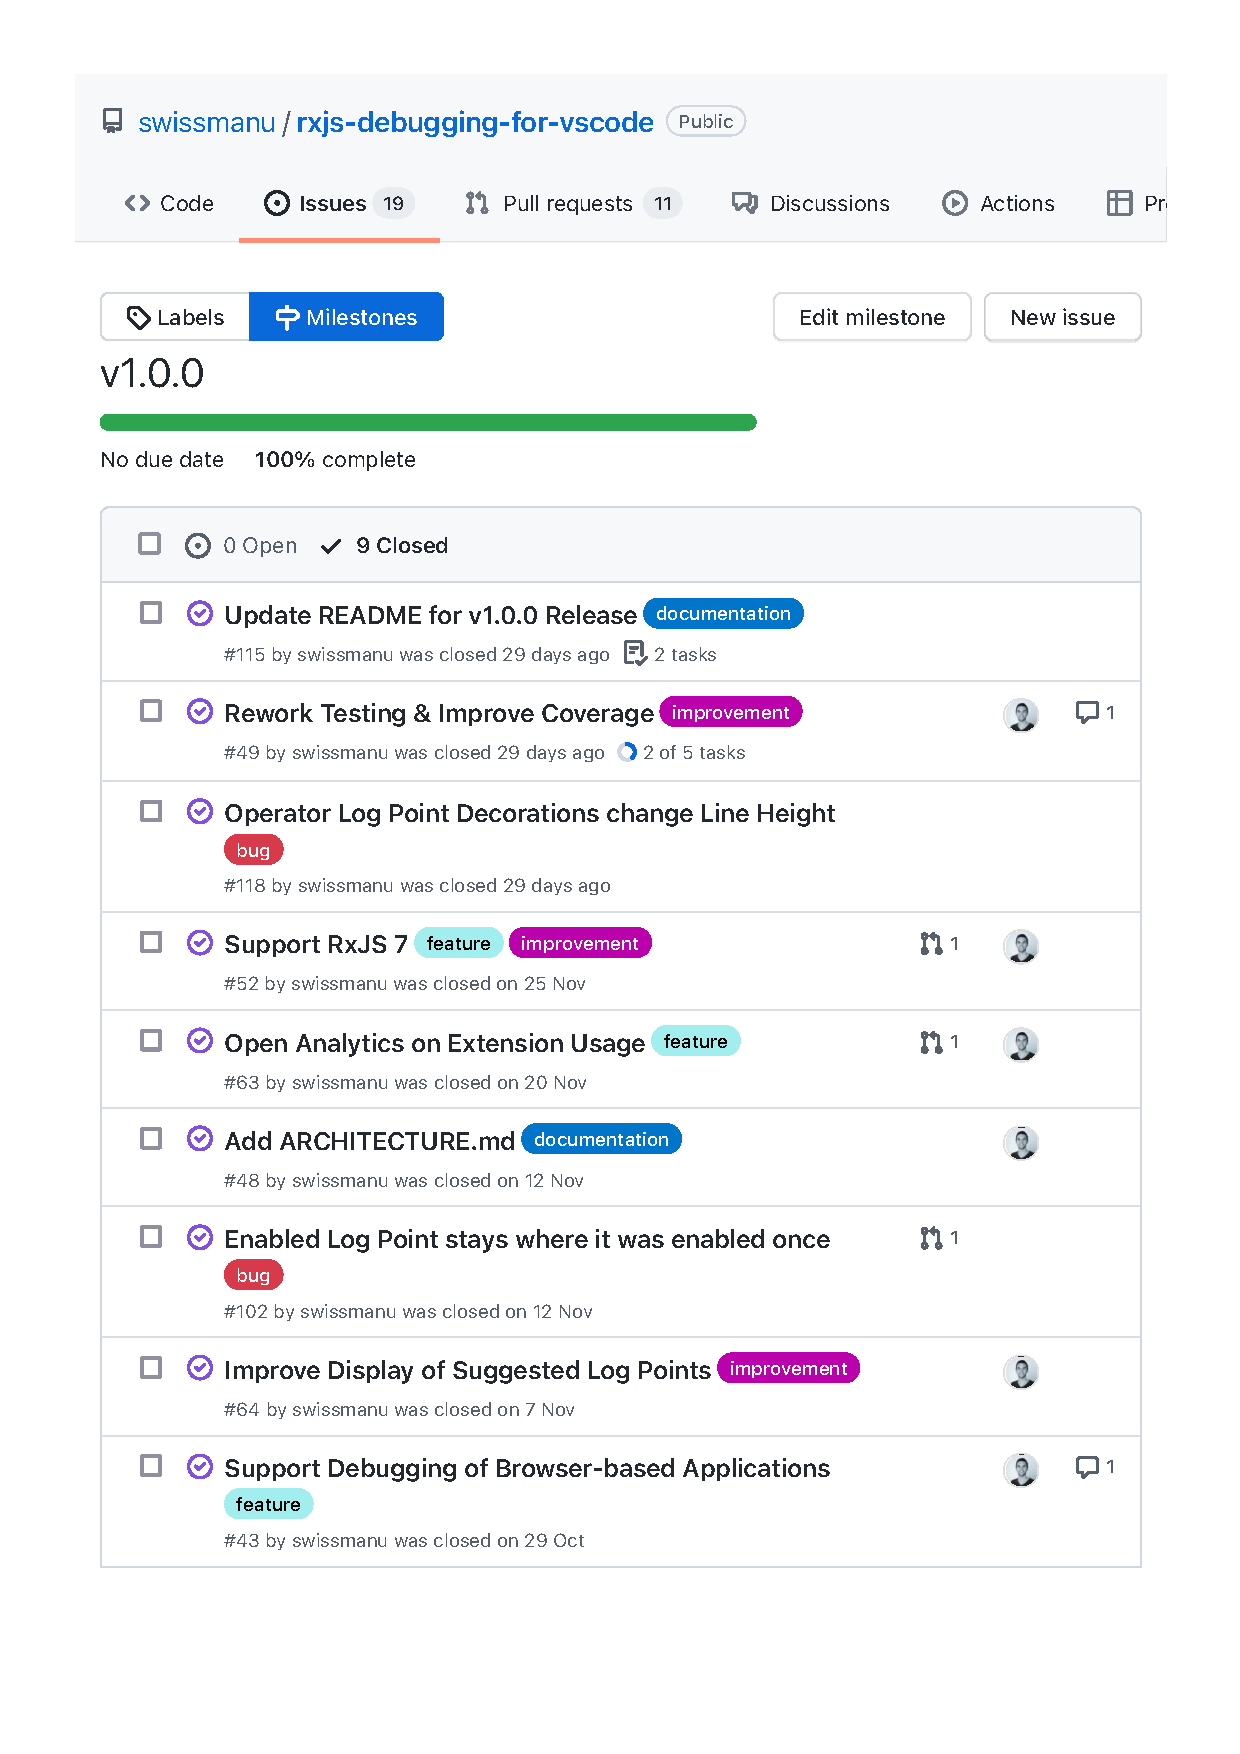
\includepdf[pages=-]{content/pdfs/major-milestone.pdf}




\subsection{Feature Backlog}
\label{sec:feature-backlog}
The following document was created at the 31th of December, 10:00 CET. Its most current version is publicly accesible:

\begin{itemize}
  \item \url{https://github.com/swissmanu/rxjs-debugging-for-vscode/issues?q=is%3Aopen+is%3Aissue+label%3Afeature%2Cimprovement}
\end{itemize}

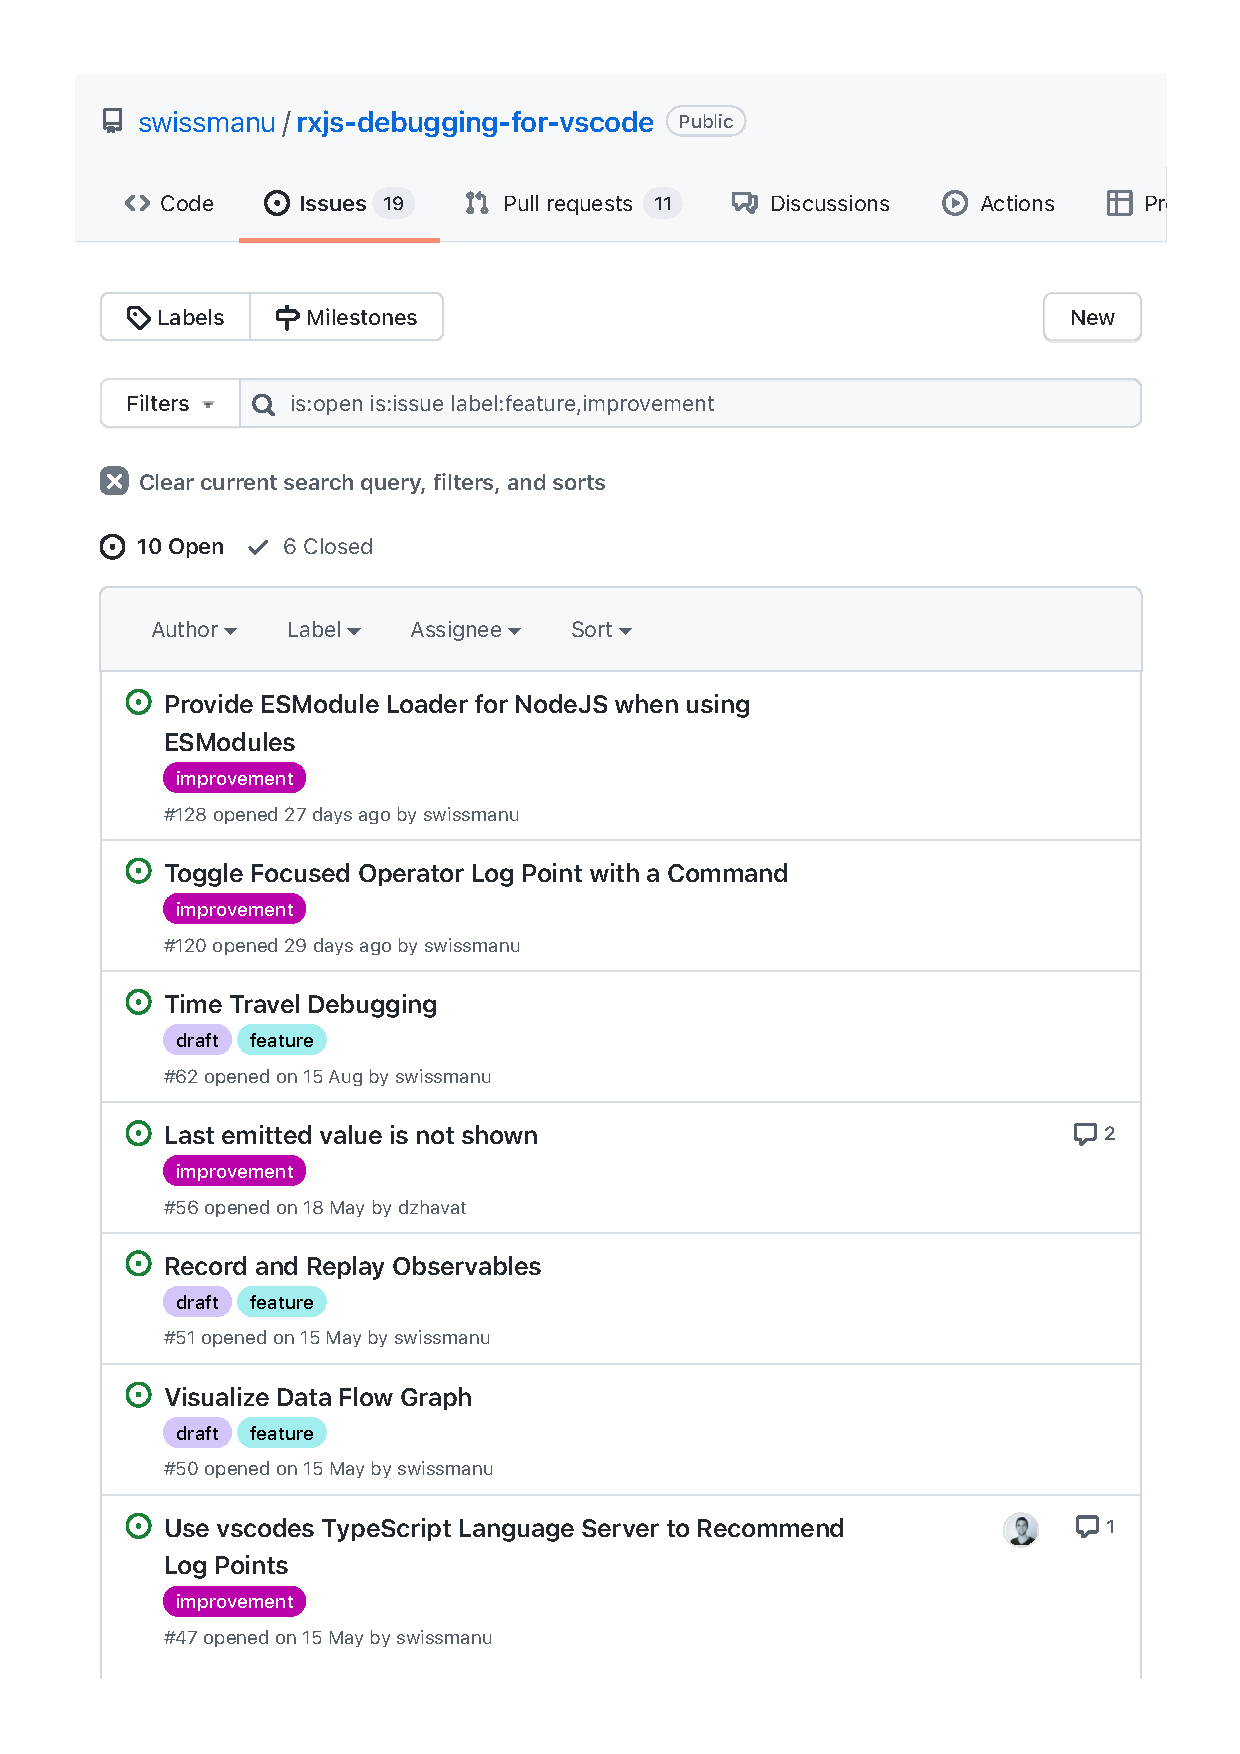
\includepdf[pages=-, landscape=true, nup=2, frame=true]{content/pdfs/feature-backlog.pdf}


\subsection{Release Tweet Stats}
\label{sec:release-tweet-stats}
The following screenshot was taken at the 30th of December, 19:00 CET.

URL of the publicly available tweet:

\begin{itemize}
  \item \url{https://twitter.com/rxjsdebugging/status/1466439953731182599}
\end{itemize}

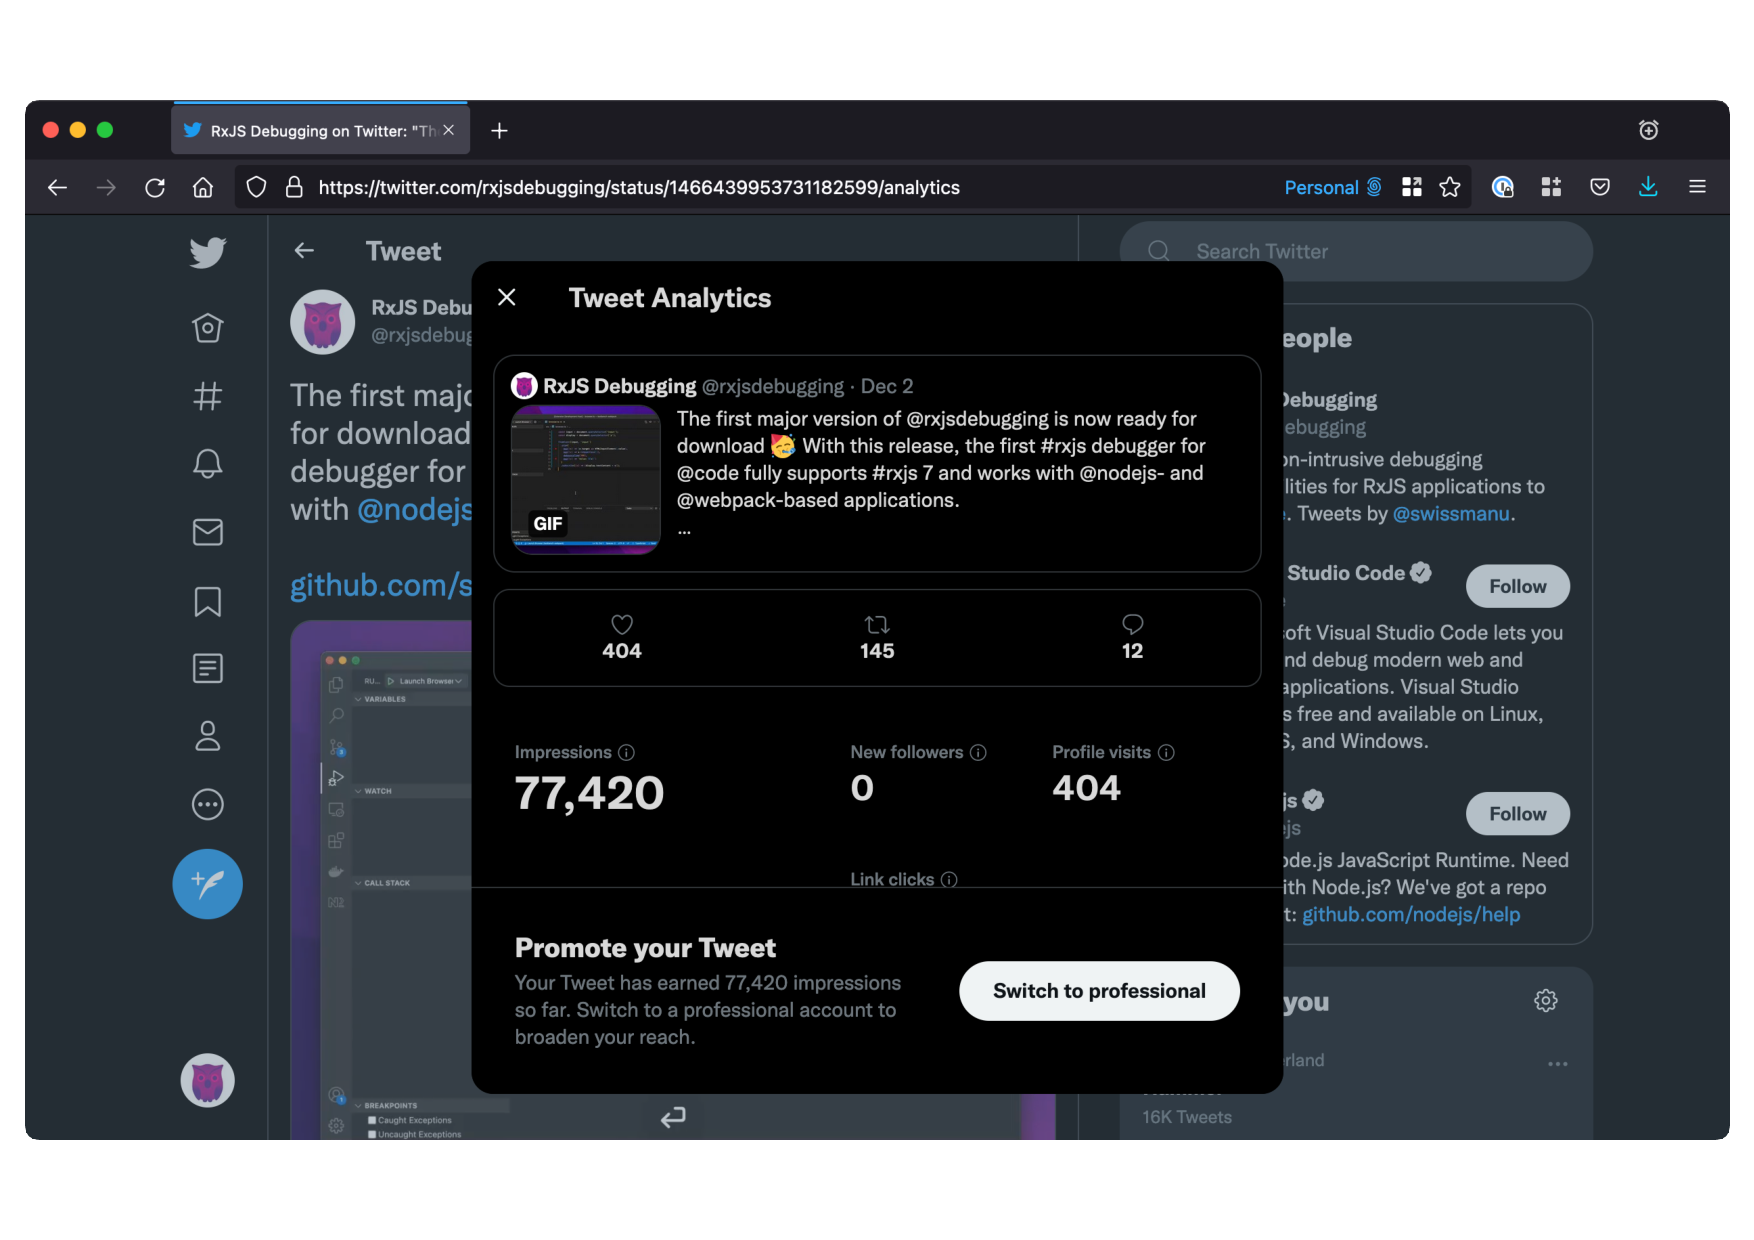
\includepdf[landscape=true,pages=-]{content/pdfs/release-tweet.pdf}


\subsection{Visual Studio Marketplace}
\label{sec:marketplace}
The following screenshots were taken at the 30th of December, 19:00 CET.

URL of the publicly available Marketplace page:

\begin{itemize}
  \item \url{https://marketplace.visualstudio.com/items?itemName=manuelalabor.rxjs-debugging-for-vs-code}
\end{itemize}

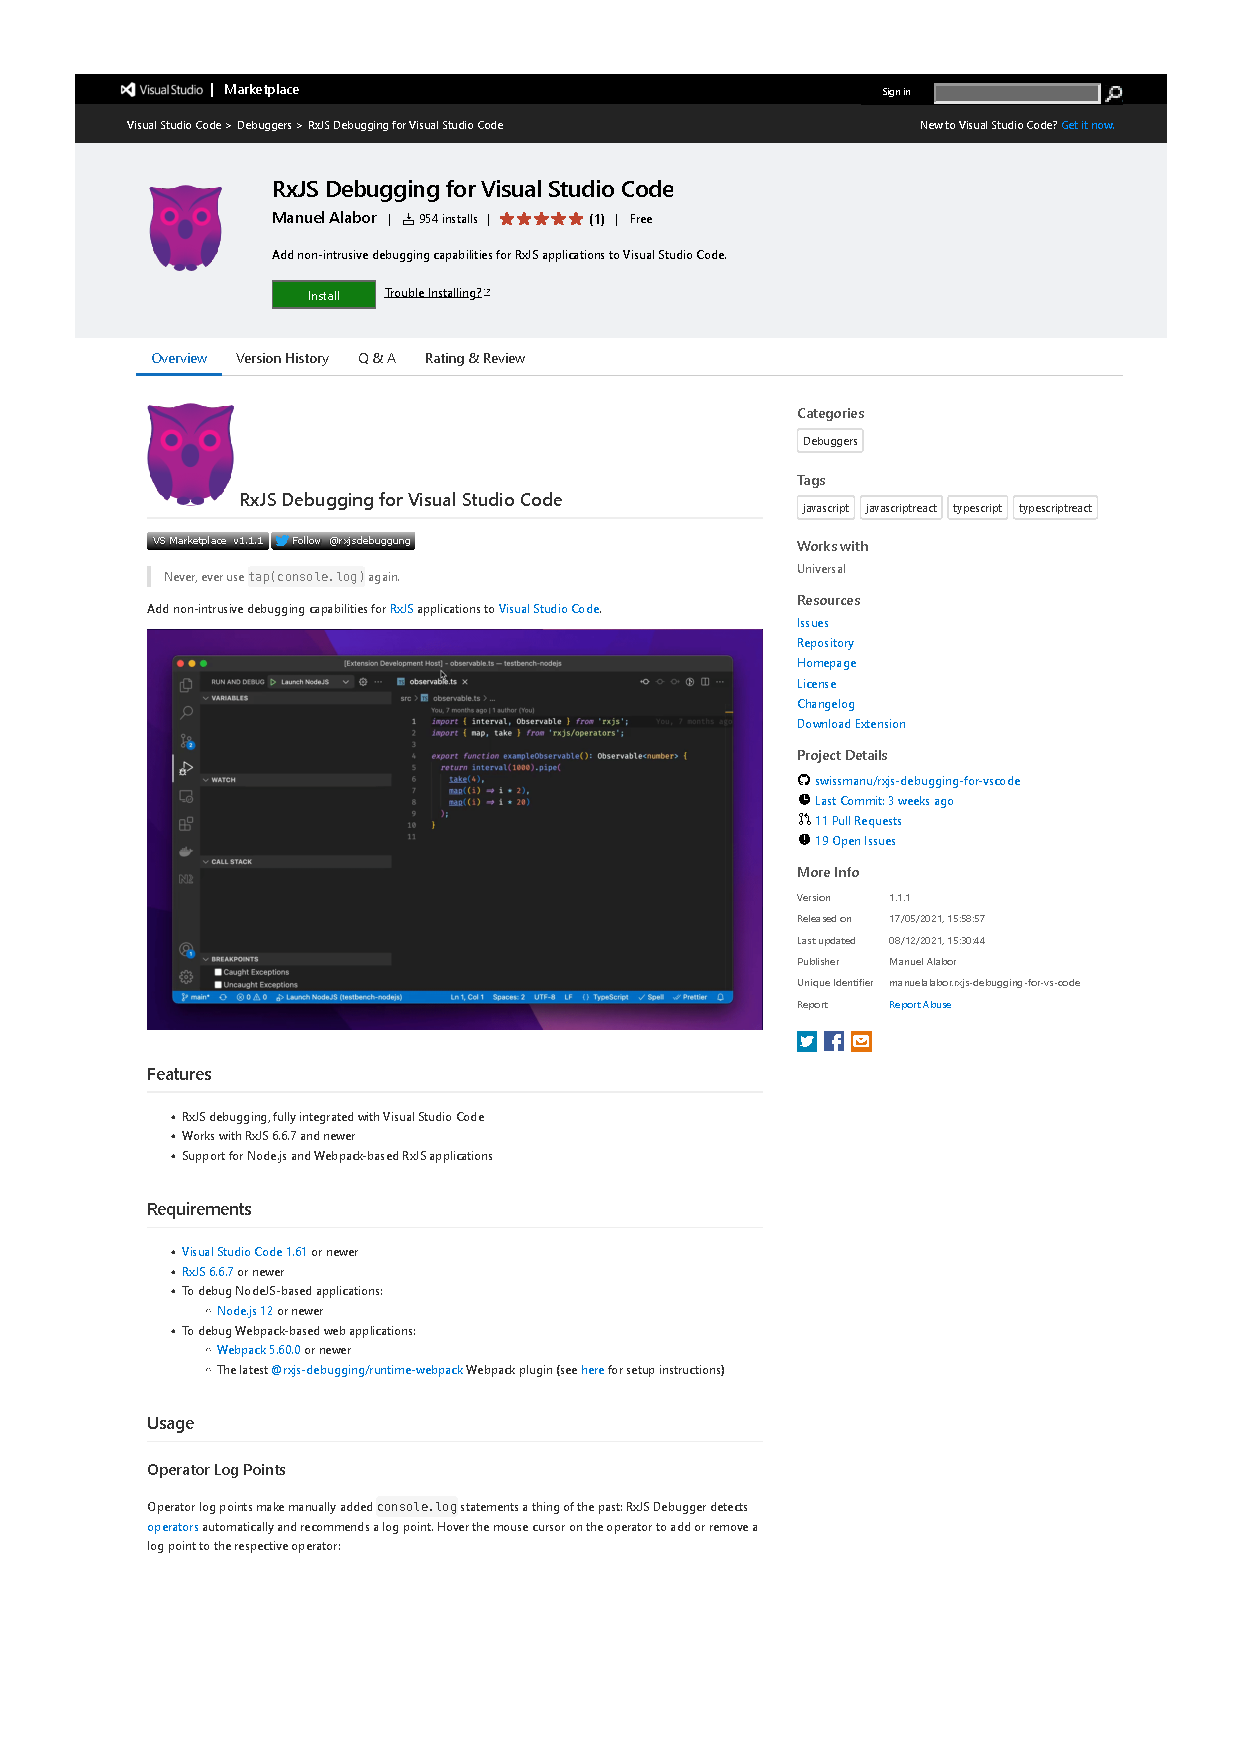
\includepdf[pages=-, landscape=true, nup=2, frame=true]{content/pdfs/marketplace.pdf}



\subsection{ANALYTICS.md}
\label{sec:analytics}
The following document is a snapshot of the ANALYTICS.md file from the Git repository of RxJS Debugging for vscode:

\begin{itemize}
  \item \url{https://github.com/swissmanu/rxjs-debugging-for-vscode/blob/1bb1c20cbf3633ef45cf0df16aacb3c3ea8a8c8c/ANALYTICS.md}
\end{itemize}

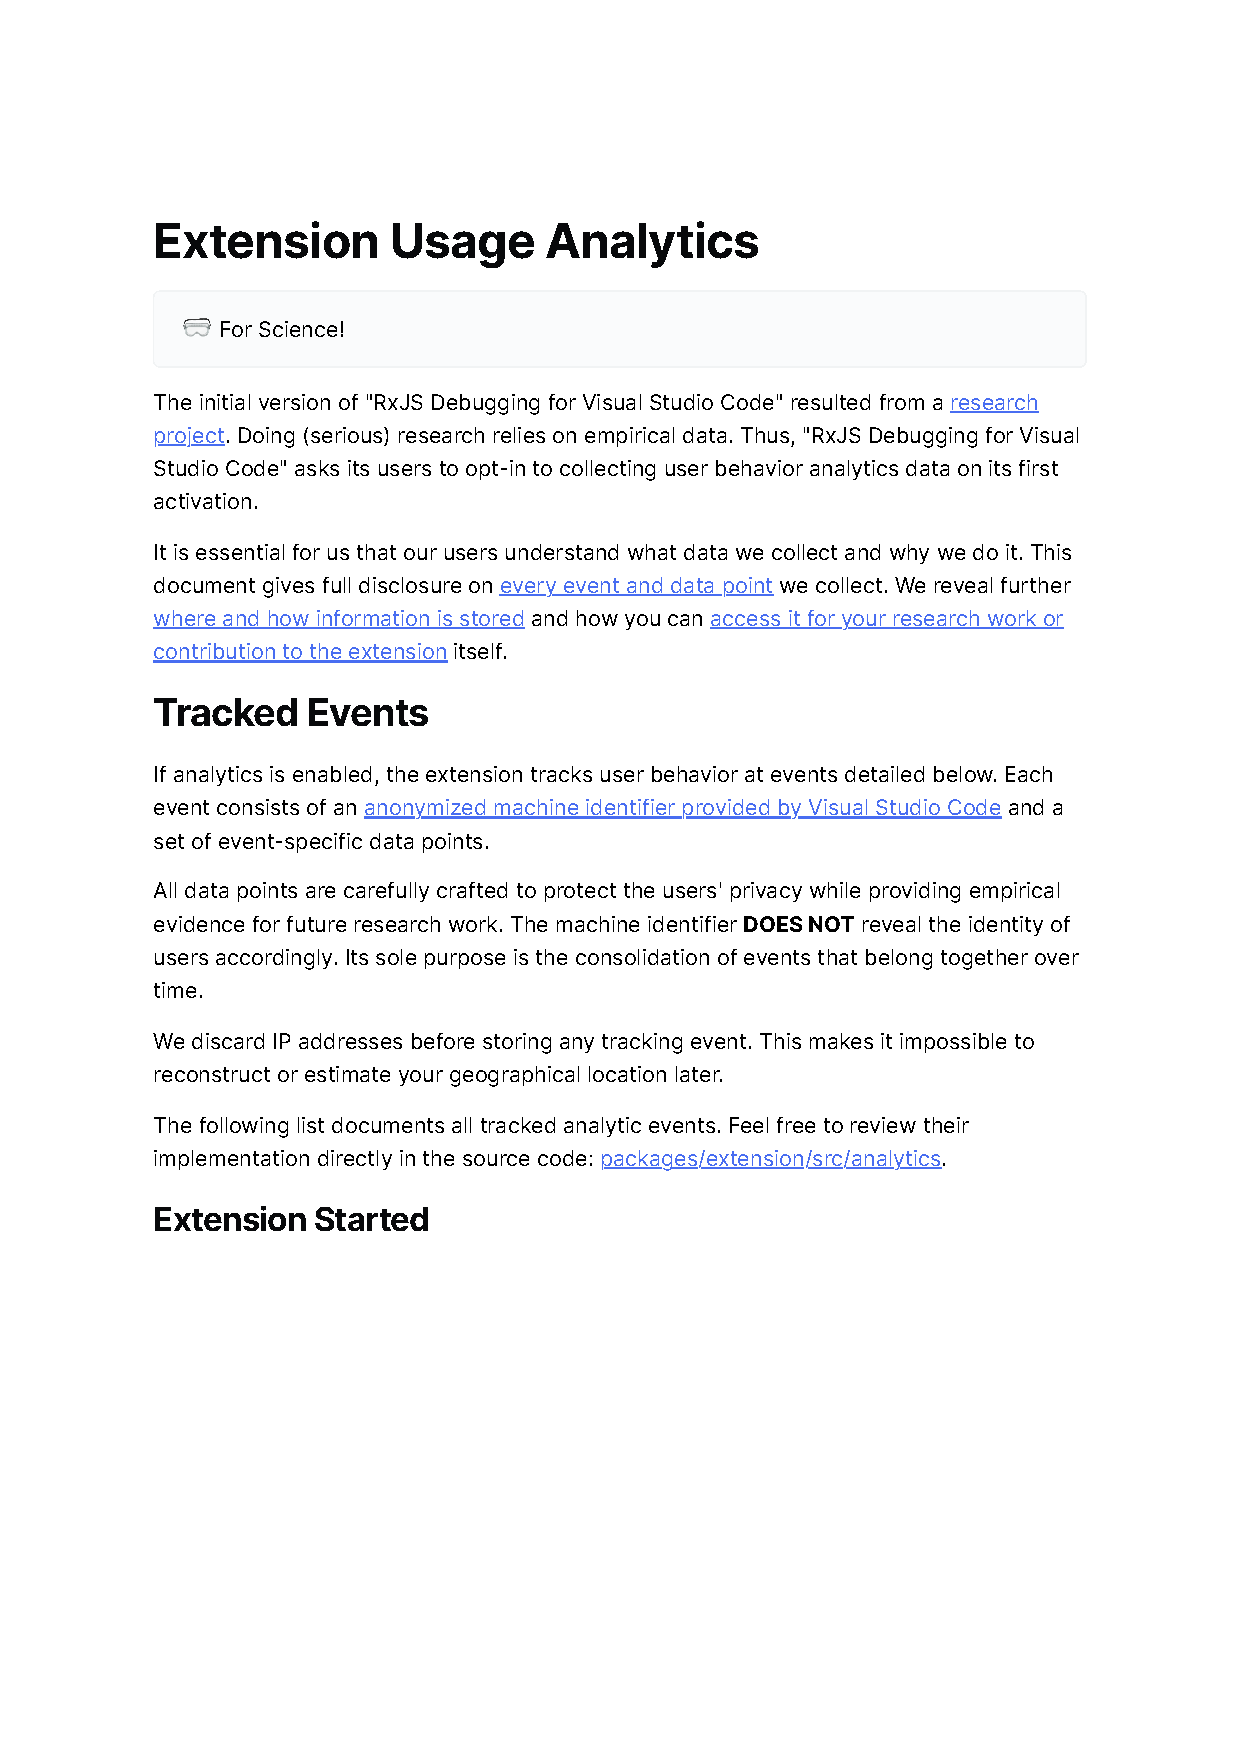
\includepdf[pages=-, landscape=true, nup=2, frame=true]{content/pdfs/analyticsmd.pdf}


\subsection{ARCHITECTURE.md}
\label{sec:architecture}
The following document is a snapshot of the ARCHITECTURE.md file from the Git repository of RxJS Debugging for vscode:

\begin{itemize}
  \item \url{https://github.com/swissmanu/rxjs-debugging-for-vscode/blob/50ca1b93427bd87e6af1a7466b46d1bf669cce6c/ARCHITECTURE.md}
\end{itemize}

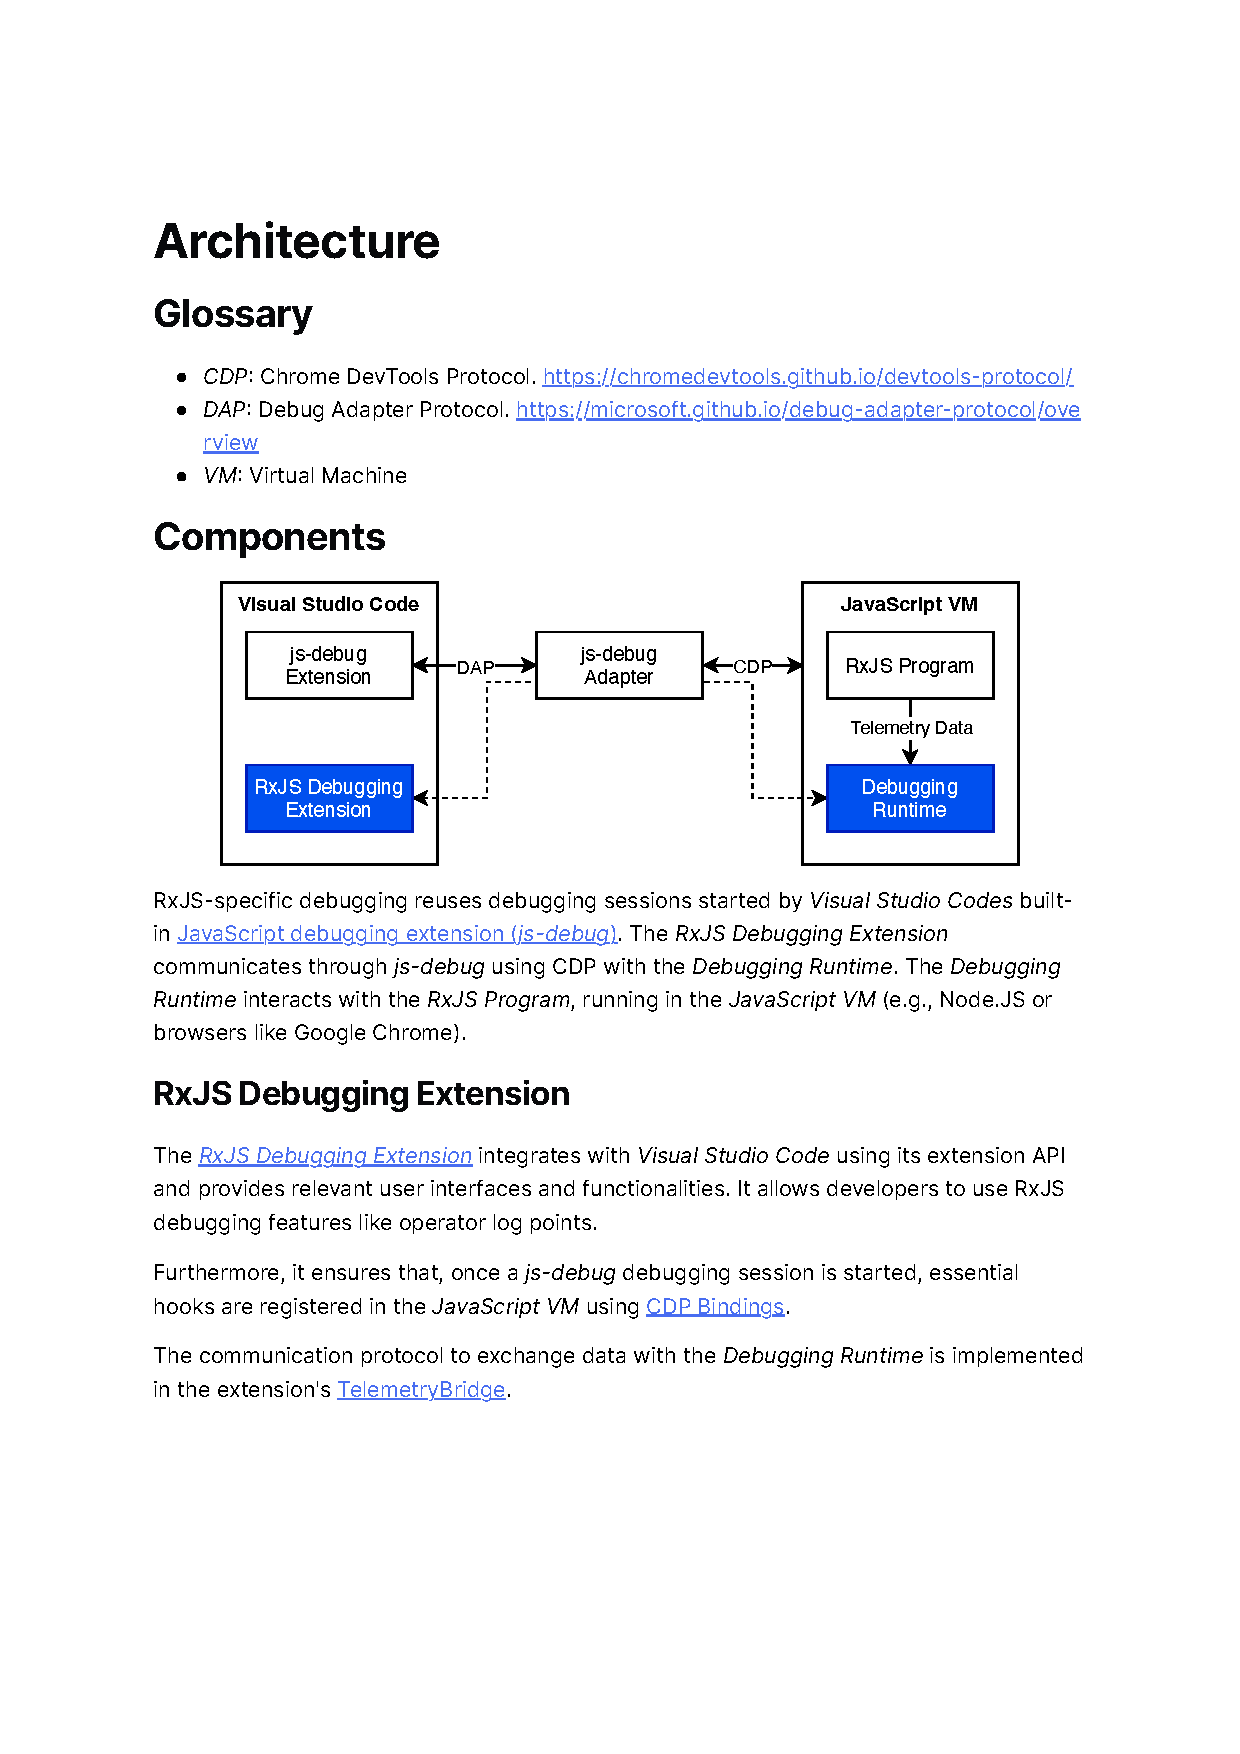
\includepdf[pages=-, landscape=true, nup=2, frame=true]{content/pdfs/architecturemd.pdf}


\subsection{CHANGELOG.md}
\label{sec:changelog}
The following document is a snapshot of the CHANGELOG.md file from the Git repository of RxJS Debugging for vscode:

\begin{itemize}
  \item \url{https://github.com/swissmanu/rxjs-debugging-for-vscode/blob/1cdb1579b872243a10747c94d9c623759dfa83f0/CHANGELOG.md}
\end{itemize}

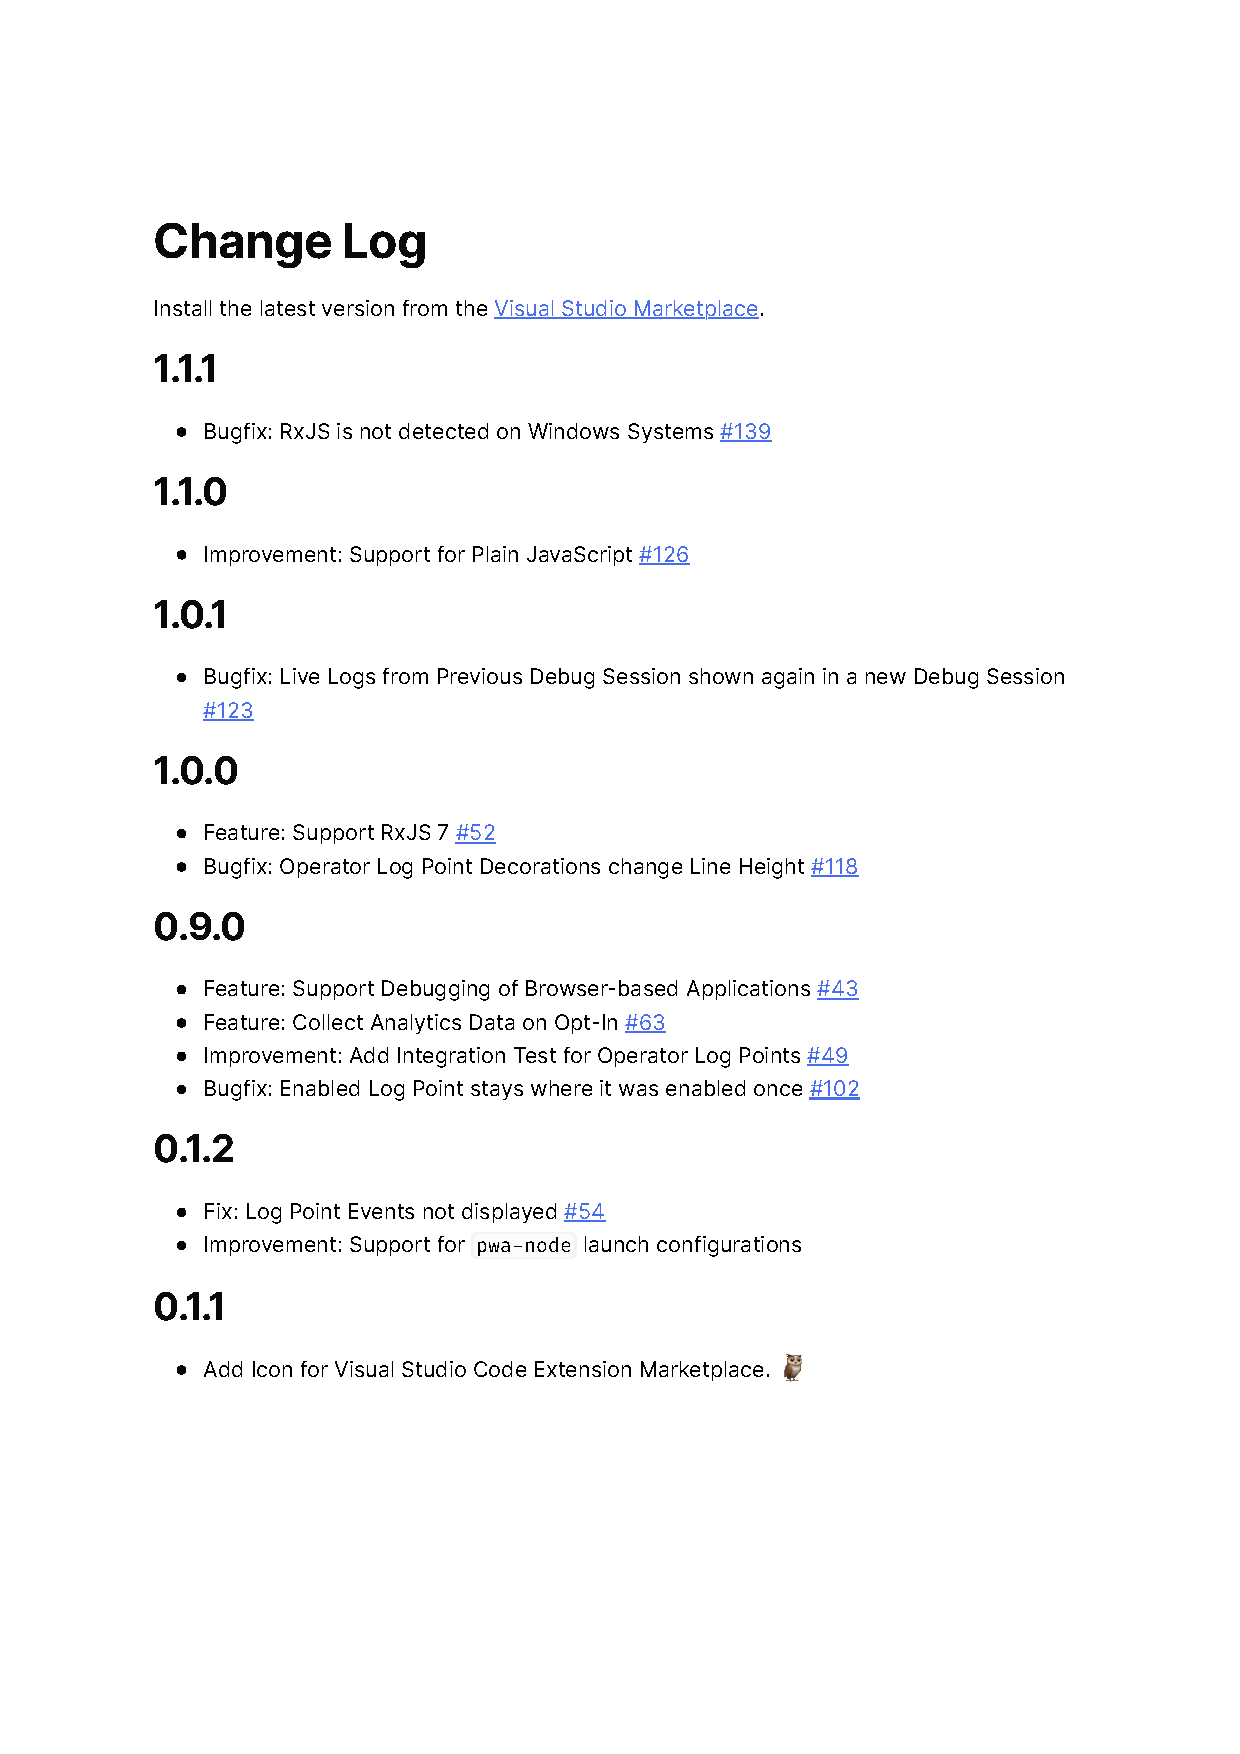
\includepdf[pages=-, landscape=true, nup=2, frame=true]{content/pdfs/changelogmd.pdf}



\subsection{CONTRIBUTING.md}
\label{sec:contributing}
The following document is a snapshot of the CONTRIBUTING.md file from the Git repository of RxJS Debugging for vscode:

\begin{itemize}
  \item \url{https://github.com/swissmanu/rxjs-debugging-for-vscode/blob/2da72e21a733c99522633d8477892f3b5b48113c/CONTRIBUTING.md}
\end{itemize}

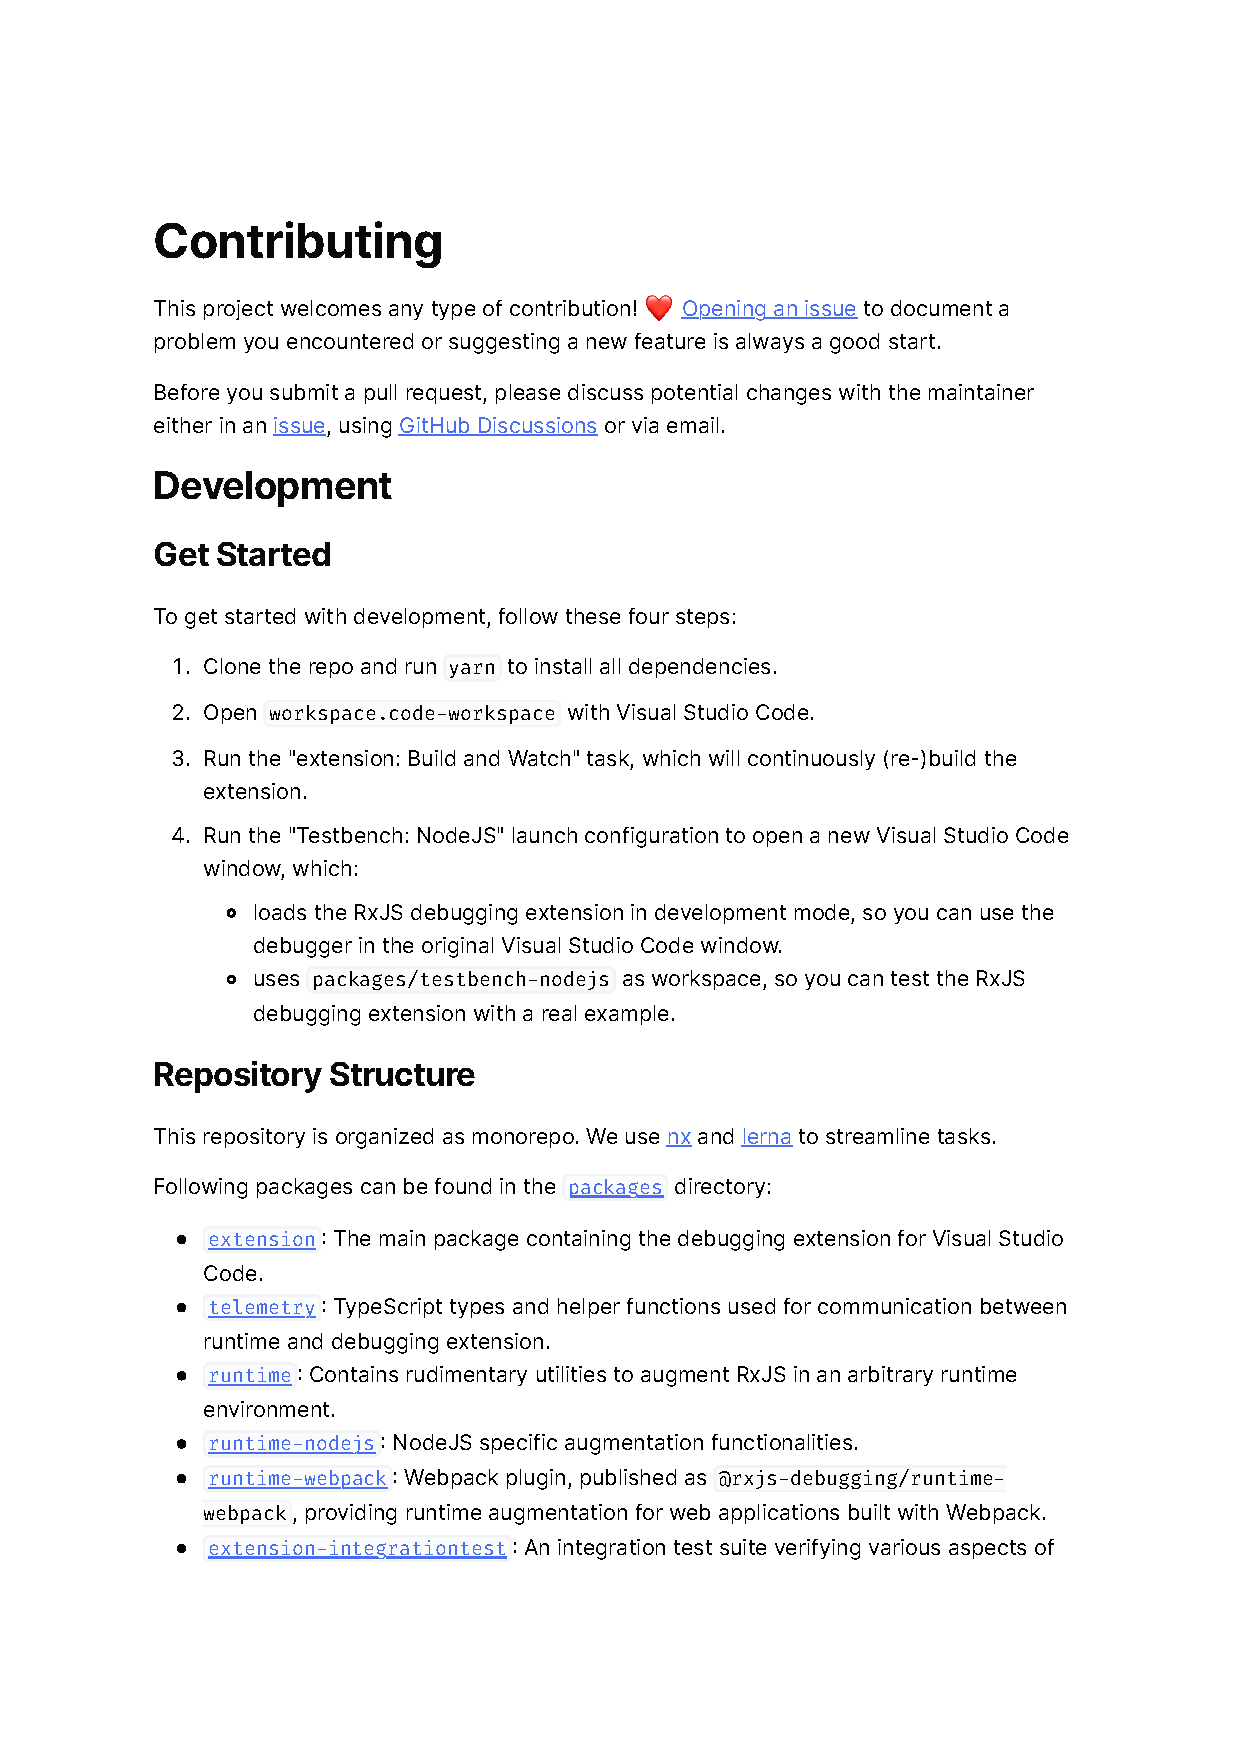
\includepdf[pages=-, landscape=true, nup=2, frame=true]{content/pdfs/contributingmd.pdf}



\subsection{Analytics Dashboard}
\label{sec:analytics-dashboard}
The following screenshot was taken at the 30th of December 2021, 19:00 CET.

As described in Appendix \ref{sec:analytics}, analytics data is not publicly accessible at this time.

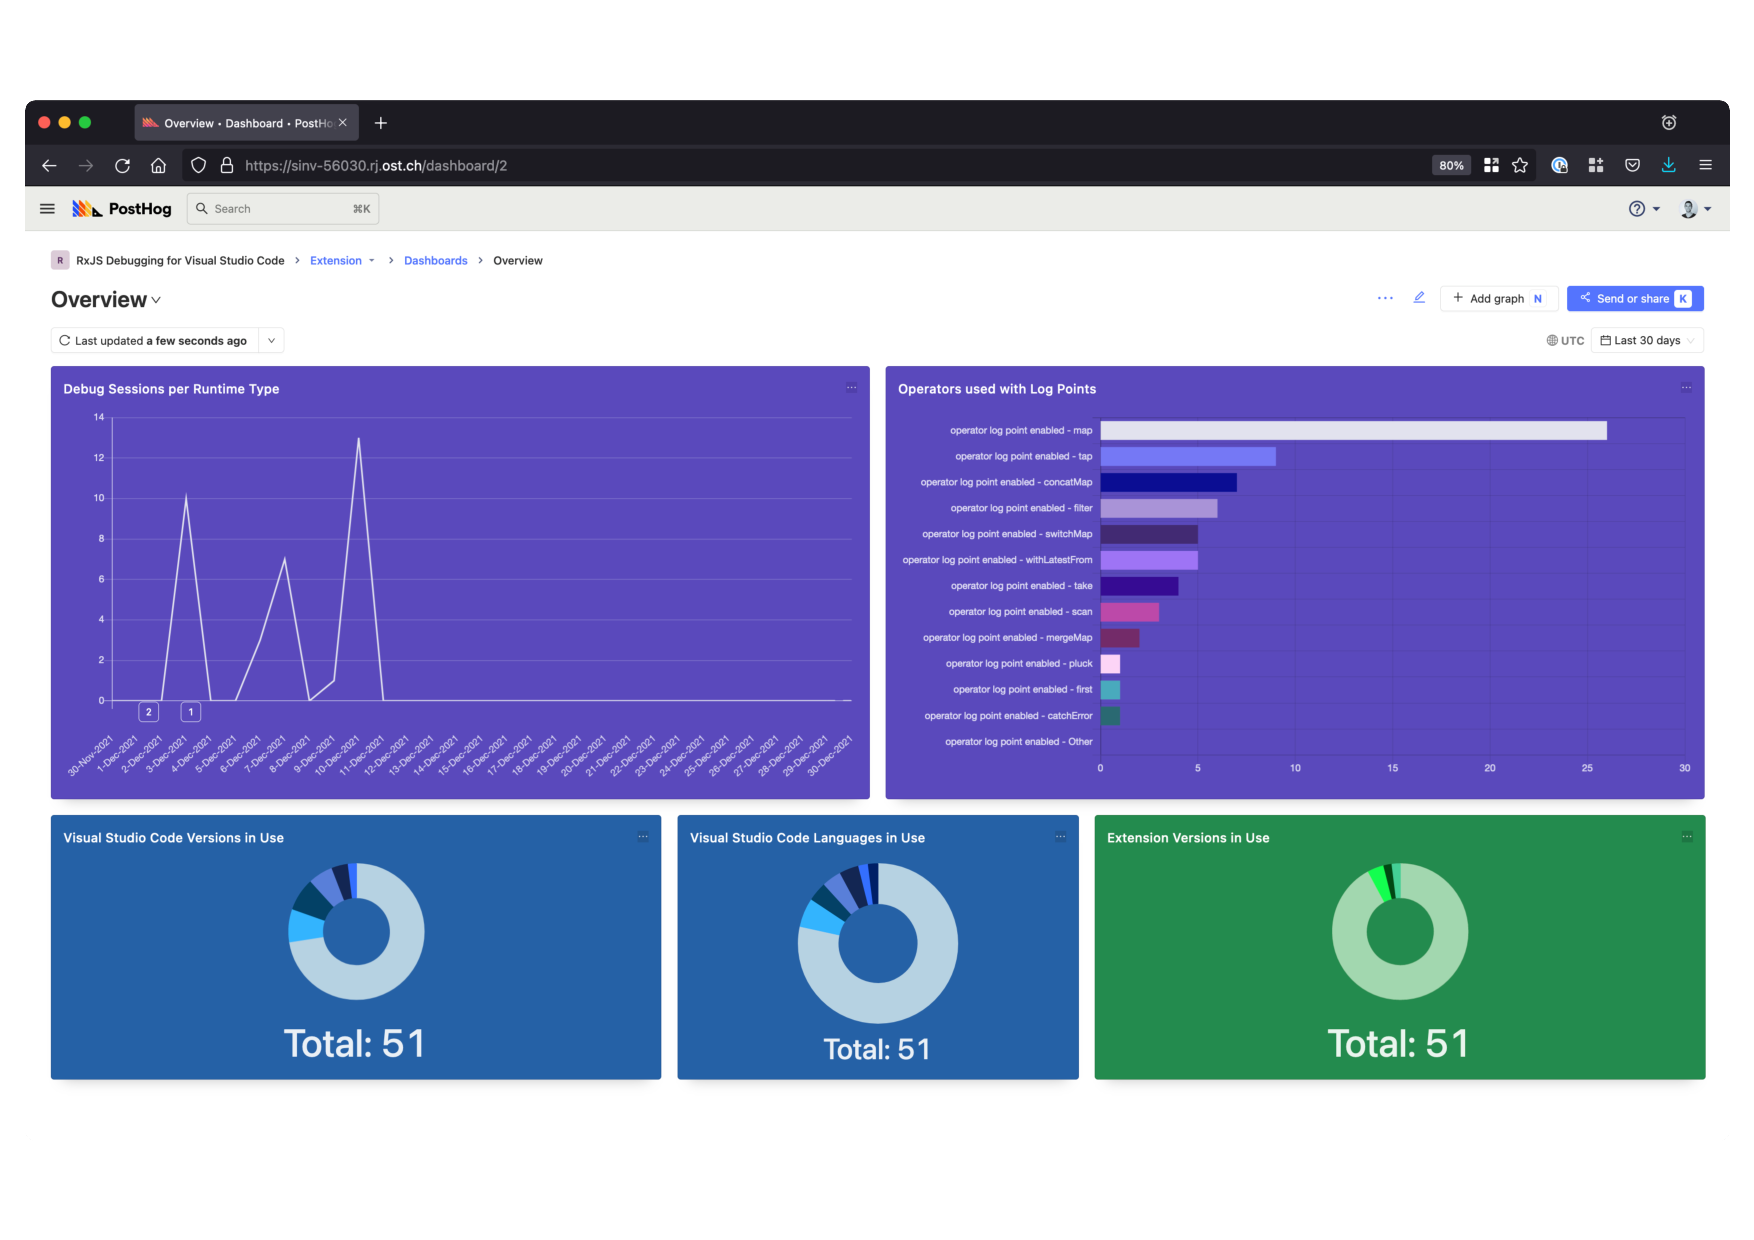
\includepdf[landscape=true, pages=-]{content/pdfs/posthog.pdf}



\section{vscode-js-debug Pull Request: Reuse CDP Connection}
\label{sec:cdp-pull-request}
The following document was created at the 31th of December, 10:00 CET and is publicly accesible:

\begin{itemize}
  \item \url{https://github.com/microsoft/vscode-js-debug/pull/964}
\end{itemize}

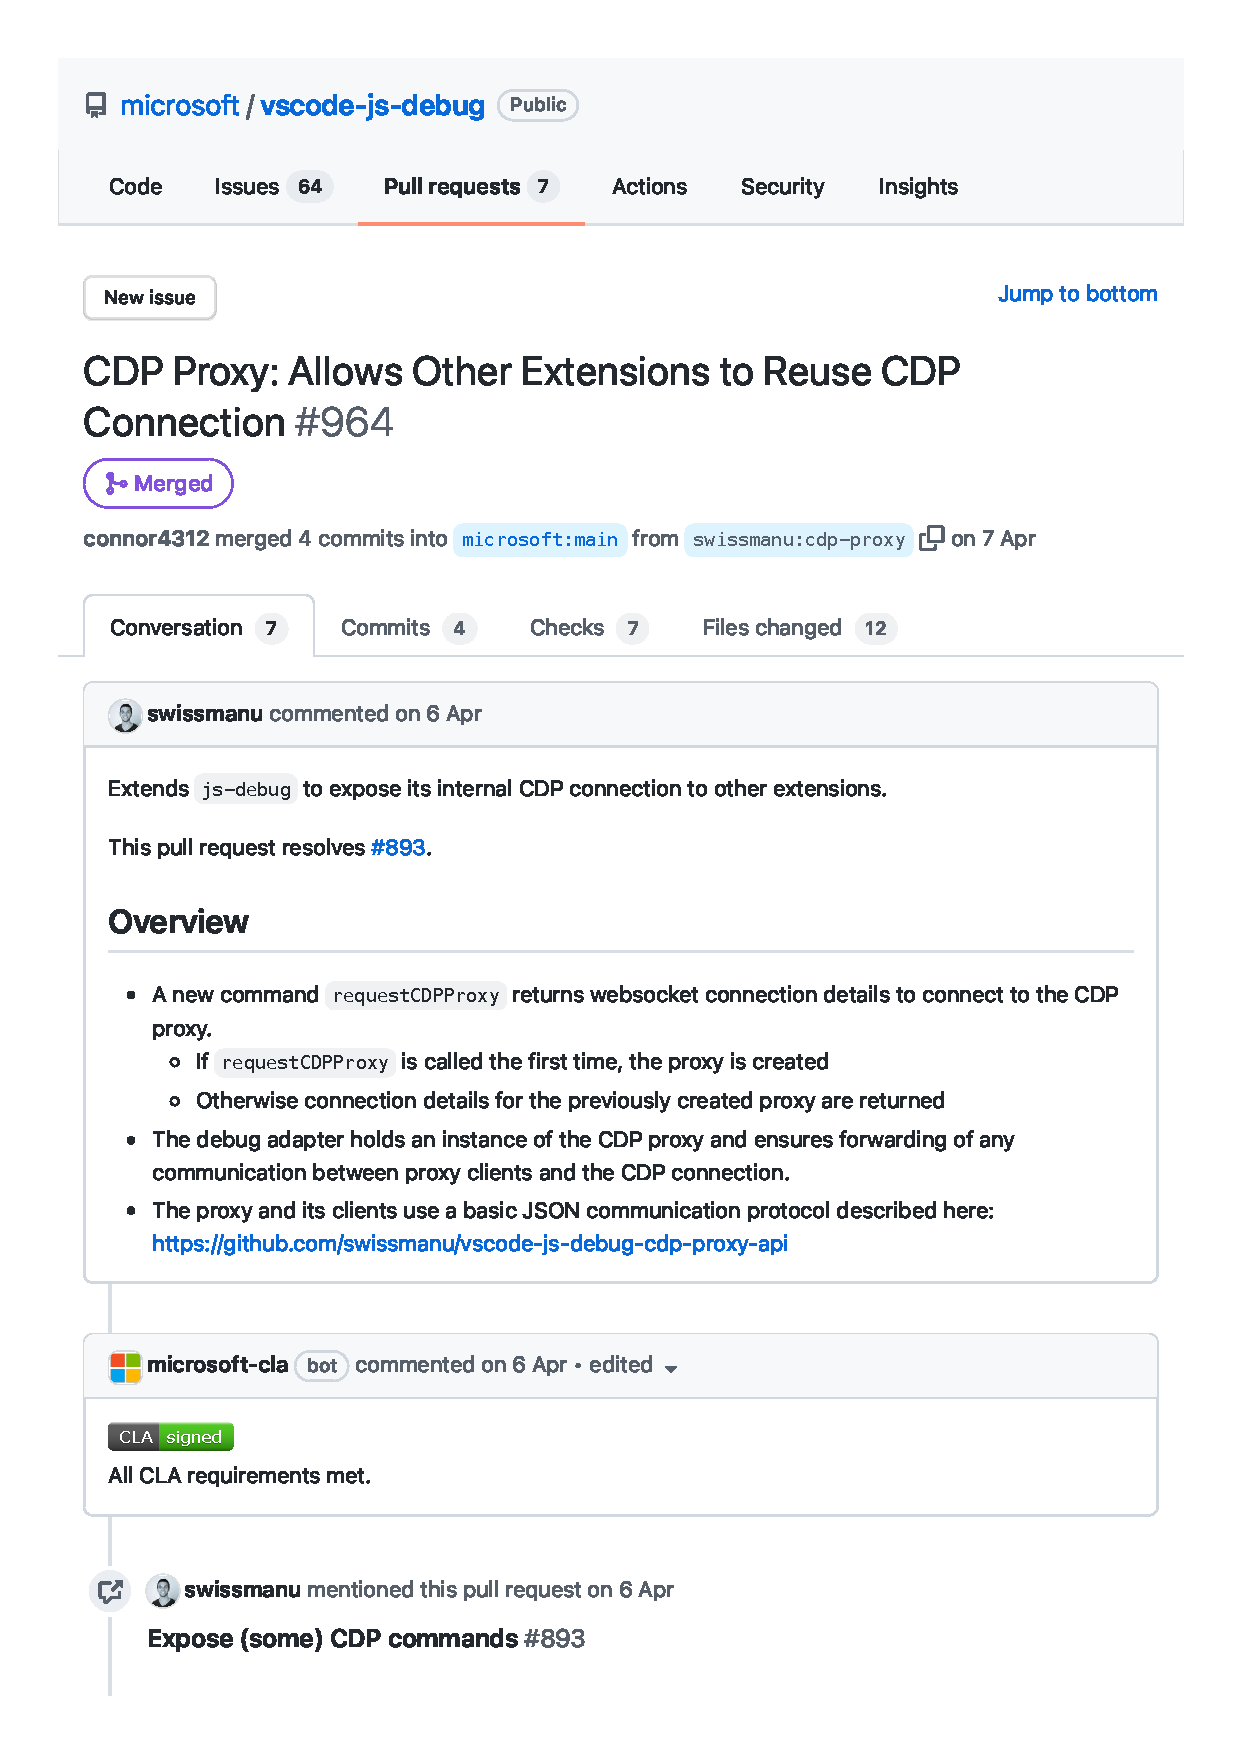
\includepdf[pages=-, landscape=true, nup=2, frame=true]{content/pdfs/cdp-pull-request.pdf}



\section{Marble Diagram Syntax}
\label{sec:marble-diagram-syntax}


\subsection*{Observables}

In a marble diagram, a horizontal arrow \raisebox{2pt}{\tikz[scale=0.35]{\draw[line width=0.4mm] (0,0) edge[->] (2,0)}} pointing from left to right represents the timeline of an observable. Such a timeline uses following depictions to show when the observable emitted an event:

\begin{itemize}
  \item A marble \raisebox{-2pt}{\tikz{\node [shape=circle, draw, line width=0.3mm, inner sep=0.6mm, font=\footnotesize] {v};}} indicates a \texttt{next} event carrying the displayed value \texttt{v}
  \item A vertical bar \raisebox{-3pt}{\tikz[scale=0.36]{\draw[line width=0.4mm] (0,0) -- (0,1);}} shows a \texttt{complete} event
  \item \texttt{next} and \texttt{complete} can take place at the same time, thus are shown as the combination of a marble and a vertical bar: \raisebox{-5pt}{\tikz{\draw[line width=0.3mm] (0,0.28) -- (0,-0.28); \node [shape=circle, draw, fill=white, line width=0.3mm, inner sep=0.6mm, font=\footnotesize] {v};}}
  \item Finally, the cross \raisebox{-3pt}{\tikz[scale=0.35]{\draw[line width=0.4mm] (0,0) -- (1,1); \draw[line width=0.4mm] (0,1) -- (1,0);}} indicates that an \texttt{error} occurred
\end{itemize}

\subsection*{Operators}

Operators project events from a source to target observable. In a marble diagram, operators are depicted using a rectangular box \raisebox{-3pt}{\tikz{\node [shape=rectangle, draw, line width=0.3mm, inner sep=0.8mm, font=\footnotesize] {operator}}}.

An event consumed by an operator is indicated with a vertical arrow \raisebox{-3pt}{\tikz[scale=0.36]{\draw[line width=0.4mm, gray, dotted] (0,1) edge[->] (0,0)}} pointing from the source observable to the operator.

An event projected to the target observable is shown using vertical arrow \raisebox{-3pt}{\tikz[scale=0.36]{\draw[line width=0.4mm, gray, dotted] (0,1) edge[->] (0,0)}} pointing from the operator to the target observable.

\subsection*{Examples}

\subsubsection*{Integers}
A simple observable emitting integers from 1 through 4 that completes eventually.

\begin{figure}[H]
  \centering
  \begin{tikzpicture}[node distance=6mm]
    \pgfdeclarelayer{edgelayer}
    \pgfdeclarelayer{nodelayer}
    \pgfsetlayers{background,edgelayer,nodelayer,main}

    \tikzstyle{marble}=[circle, draw, fill=white, line width=0.3mm, inner sep=2mm, font=\small]
    \tikzstyle{operator}=[rectangle, draw, fill=white, line width=0.3mm, inner sep=2mm, minimum width=120mm, xshift=-5mm]
    \tikzstyle{observable}=[->, line width=0.3mm]
    \tikzstyle{complete}=[line width=0.3mm]
    \tikzstyle{project}=[->, dotted, gray, line width=0.3mm]

    \begin{pgfonlayer}{nodelayer}
        \node (1) [style=marble] {1};
        \node (2) [style=marble, right=of 1] {2};
        \node (3) [style=marble, right=of 2] {3};
        \node (4) [style=marble, right=of 3] {4};
    \end{pgfonlayer}

    \begin{pgfonlayer}{edgelayer}
        \draw ($(1)   -(9mm,0)$)      edge[style=observable]   ($(4)    +(14.5mm,0)$);
        \draw ($(4)   +(+9mm,0) -(0,4mm)$)  edge[style=complete] ($(4)   +(+9mm,4mm)$);
    \end{pgfonlayer}
  \end{tikzpicture}
\end{figure}

\subsubsection*{Operator}

A marble diagram showing a source observable emitting the integers from 1 through 6. The source completes immediately after its last value was emitted. The \texttt{take} operator projects the first four values and then completes the target observable.

\begin{figure}[H]
  \centering
  \begin{tikzpicture}[node distance=6mm]
      \pgfdeclarelayer{edgelayer}
      \pgfdeclarelayer{nodelayer}
      \pgfsetlayers{background,edgelayer,nodelayer,main}

      \tikzstyle{marble}=[circle, draw, fill=white, line width=0.3mm, inner sep=2mm,
      font=\small]
      \tikzstyle{operator}=[rectangle, draw, fill=white, line width=0.3mm, inner sep=2mm, minimum width=90mm, xshift=-5mm]
      \tikzstyle{observable}=[->, line width=0.3mm]
      \tikzstyle{complete}=[line width=0.3mm]
      \tikzstyle{project}=[->, dotted, gray, line width=0.3mm]

      \begin{pgfonlayer}{nodelayer}
          \node (1) [style=marble] {1};
          \node (2) [style=marble, right=of 1] {2};
          \node (3) [style=marble, right=of 2] {3};
          \node (4) [style=marble, right=of 3] {4};
          \node (5) [style=marble, right=of 4] {5};
          \node (6) [style=marble, right=of 5] {6};

          \node (filter) [style=operator, below=13mm of 1.west, anchor=west] {take(4)};

          \node (1_t) [style=marble, below=17mm of 1] {1};
          \node (2_t) [style=marble, below=17mm of 2] {2};
          \node (3_t) [style=marble, below=17mm of 3] {3};
          \node (4_t) [style=marble, below=17mm of 4] {4};

      \end{pgfonlayer}

      \begin{pgfonlayer}{edgelayer}
          \draw ($(1)   -(9mm,0)$)    edge[style=observable]   ($(6)    +(8.5mm,0)$);
          \draw ($(1_t) -(9mm,0)$)    edge[style=observable]   ($(4_t)  +(37.5mm,0)$);

          \draw (1)                   edge[style=project]     ($(1) -(0,9mm)$);
          \draw (2)                   edge[style=project]     ($(2) -(0,9mm)$);
          \draw (3)                   edge[style=project]     ($(3) -(0,9mm)$);
          \draw (4)                   edge[style=project]     ($(4) -(0,9mm)$);
          \draw (5)                   edge[style=project]     ($(5) -(0,9mm)$);
          \draw (6)                   edge[style=project]     ($(6) -(0,9mm)$);

          \draw ($(1_t) +(0,9mm)$)    edge[style=project]     (1_t);
          \draw ($(2_t) +(0,9mm)$)    edge[style=project]     (2_t);
          \draw ($(3_t) +(0,9mm)$)    edge[style=project]     (3_t);
          \draw ($(4_t) +(0,9mm)$)    edge[style=project]     (4_t);

          \draw ($(6) -(0,6mm)$)      edge[style=complete]    ($(6) +(0,6mm)$);
          \draw ($(4_t) -(0,6mm)$)    edge[style=complete]    ($(4_t) +(0,6mm)$);
      \end{pgfonlayer}
  \end{tikzpicture}
\end{figure}

\subsubsection*{Error}

The following marble diagrams shows an observable that failed with an \texttt{error} event after it emitted the integers 1 and 2.

\begin{figure}[H]
  \centering
  \begin{tikzpicture}[node distance=6mm]
    \pgfdeclarelayer{edgelayer}
    \pgfdeclarelayer{nodelayer}
    \pgfsetlayers{background,edgelayer,nodelayer,main}

    \tikzstyle{marble}=[circle, draw, fill=white, line width=0.3mm, inner sep=2mm, font=\small]
    \tikzstyle{operator}=[rectangle, draw, fill=white, line width=0.3mm, inner sep=2mm, minimum width=120mm, xshift=-5mm]
    \tikzstyle{observable}=[->, line width=0.3mm]
    \tikzstyle{complete}=[line width=0.3mm]
    \tikzstyle{project}=[->, dotted, gray, line width=0.3mm]

    \begin{pgfonlayer}{nodelayer}
        \node (1) [style=marble] {1};
        \node (2) [style=marble, right=of 1] {2};
    \end{pgfonlayer}

    \begin{pgfonlayer}{edgelayer}
        \draw ($(1)   -(9mm,0)$)      edge[style=observable]   ($(2)    +(18.5mm,0)$);
        \draw ($(2)   +(+8mm,0) -(0,3mm)$)  edge[style=complete] ($(2)   +(+14mm,3mm)$);
        \draw ($(2)   +(+14mm,0) -(0,3mm)$)  edge[style=complete] ($(2)   +(+8mm,3mm)$);
    \end{pgfonlayer}
  \end{tikzpicture}
\end{figure}


\newpage



\section{Open Science}
\label{sec:open-science}

\subsection{This Thesis}
\begin{itemize}
  \item \url{https://github.com/swissmanu/mse-thesis} \\ (publicly accessible after May 2022)
\end{itemize}

\subsection{Research Papers}
\begin{itemize}
  \item Debugging of RxJS-based Applications \\ \url{https://github.com/swissmanu/mse-paper-debugging-of-rxjs-based-applications}
  \item Debugging Support for Reactive Programming: Feasibility of a Ready-to-hand Debugger for RxJS \\ \url{https://github.com/swissmanu/mse-paper-rxjs-debugger} \\ (publicly accessible after May 2022)
\end{itemize}

\subsection{Studies}
\begin{itemize}
  \item Observational study \\ \url{https://github.com/swissmanu/mse-pa1-experiment}
  \item Usability test \\ \url{https://github.com/swissmanu/mse-pa2-usability-test}
\end{itemize}

\subsection{User Behavior Data ``RxJS Debugging for vscode''}

Please follow the steps described on the linked page below to get access to the user behavior data set.

\begin{itemize}
  \item \url{https://github.com/swissmanu/rxjs-debugging-for-vscode/blob/main/ANALYTICS.md\#open-source-open-research-and-open-data}
\end{itemize}
